\section{System Context Diagram}

\subsection{System Boundary}

The system boundary contains the rental marketplace application and its business capabilities: account access, accommodation publication and discovery, reservation management, messaging, support, administration, and audit records. Payment processing, map/geolocation resolution, and the delivery of external notifications are represented as external systems. The identity capability is implemented inside the proposed architecture, although Delivery 1 also described an external authentication service as a possible integration. In this design, authentication is internal; an external identity provider could be added later without changing the business service boundaries.

The following diagram presents the interaction among the users and external actors, as seen in the Delivery 1, interacting with the application. For this interactions, the application will be taken as a single black box system.

\begin{figure}[H]
    \centering
    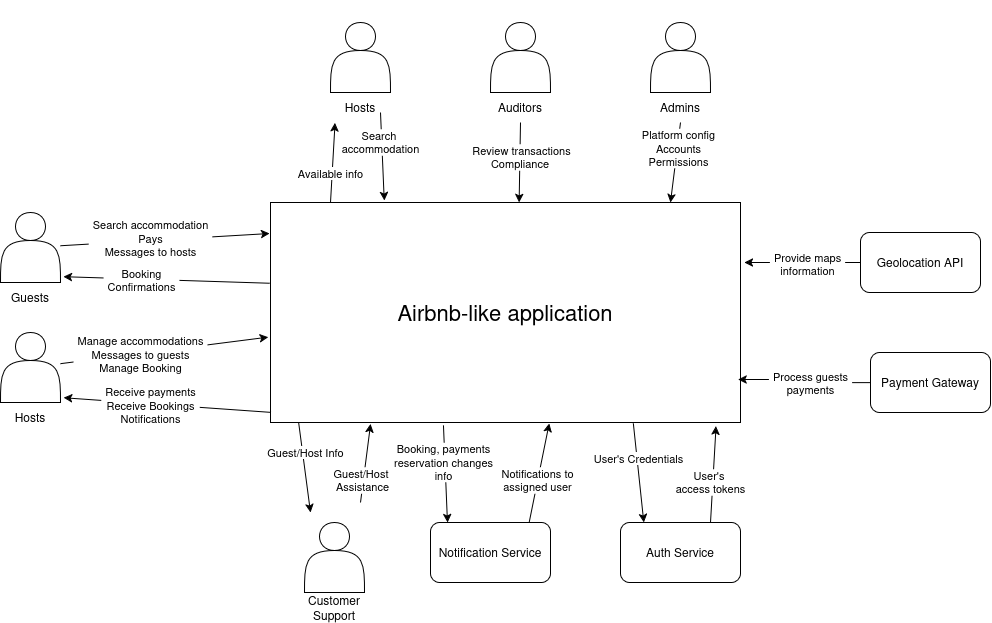
\includegraphics[width=1\linewidth]{images/SystemContextDiagram.png}
    \caption{System Context Diagram. C4 Level 1.}
    \label{fig:systemcontextdiagram}
\end{figure}
